\section{Grain structure}

A specimen is a disk (default \SI{100}{mm} diameter, \SI{35}{mm}
thick) filled with a Voronoi tessellation of grains. The builder
(\cmd{sim/core/specimen.py}, \cmd{DiskSpecimen}) controls grain count,
the spread of grain sizes about the mean (a coefficient of variation
on the seed weighting), and the random seed, so specimens are exactly
repeatable. The tessellation is rasterised onto the solver grid as a
label field: every cell carries the integer index of its grain, and
all per-grain properties (orientation, stiffness) are looked up
through that label. This label-indexed representation is what makes
the anisotropic solver practical: the stiffness tensor field never
exists in memory, only labels and a per-grain property table.

The builder also reports the diagnostics that matter physically:
achieved grain count and mean equivalent diameter, the orientation
tensor eigenvalues of the realised fabric, and the mean disorientation
across grain boundaries, which is the quantity that drives scattering
strength. The title page shows a 3D rendering of a 300-grain specimen
with each grain coloured by its in-plane c-axis azimuth;
Figure~\ref{fig:specimen-slice} shows the same specimen's mid-plane
slice.

\begin{figure}[htb]
  \centering
  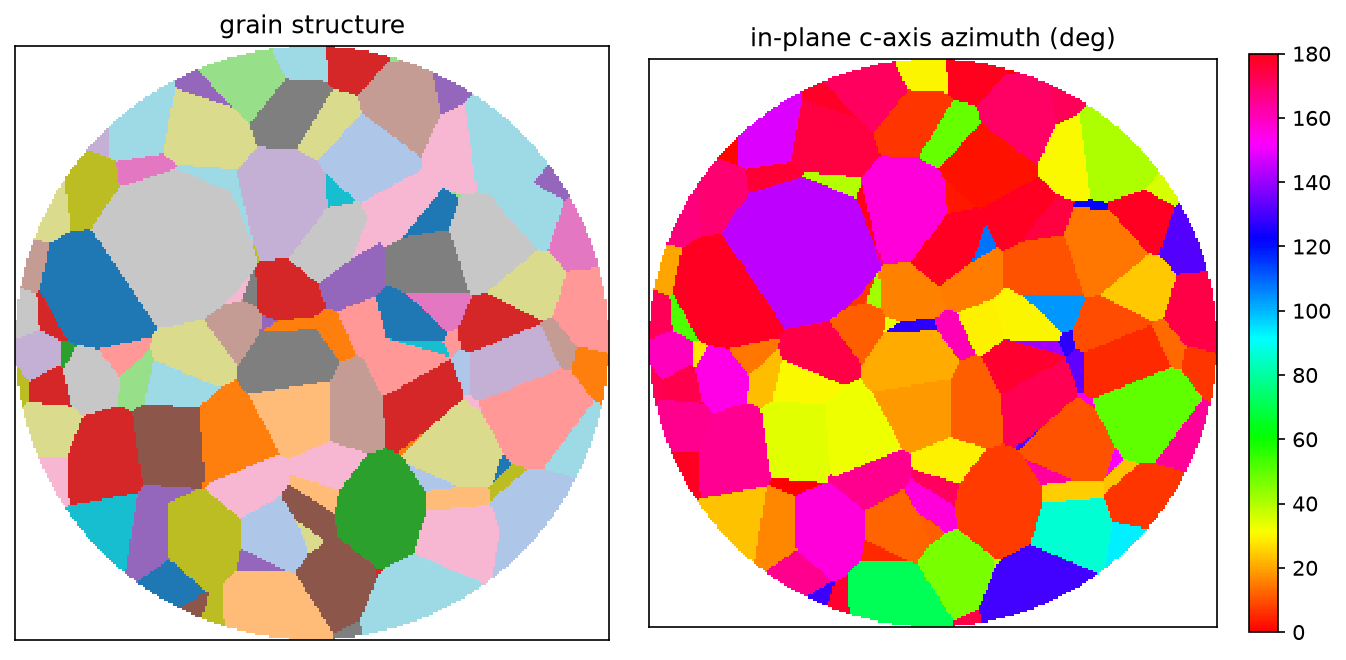
\includegraphics[width=0.95\textwidth]{figures/specimen-fabric.png}
  \caption{Mid-plane slice of a 300-grain specimen: grain structure
    (left) and the in-plane c-axis azimuth field (right).}
  \label{fig:specimen-slice}
\end{figure}
